\IEEEoverridecommandlockouts
\overrideIEEEmargins

\usepackage{amsmath,amssymb,amsfonts}
\usepackage{graphicx}
\usepackage{booktabs}
\usepackage{array}
\usepackage{microtype}
\usepackage{url}
\usepackage{cite}

\graphicspath{{figures/}}
\newcommand{\method}{CPMD}
\newcommand{\ours}{\textsc{CPMD}}
\newcommand{\R}{\mathbb{R}}
\newcommand{\Log}{\operatorname{Log}}
\newcommand{\softplus}{\operatorname{softplus}}
\newcommand{\triu}{\Pi_{<}}

\setlength{\dbltextfloatsep}{7pt plus 1pt minus 2pt}
\setlength{\textfloatsep}{7pt plus 1pt minus 2pt}
\setlength{\abovecaptionskip}{3pt}
\setlength{\belowcaptionskip}{0pt}

\title{Context-Preserving Motion Differentials\\
for Adversarial Motion Imitation}

\author{Anonymous Authors}

\begin{document}
\maketitle
\thispagestyle{empty}
\pagestyle{empty}

\begin{abstract}
Physics-based motion imitation requires a controller to match not only a
reference pose, but also the motion that produced it.  Paired tracking rewards
usually subtract the simulated state from the reference before scoring the
error.  This preserves correspondence but removes shared motion context: two
reference--policy pairs with the same differential become indistinguishable,
even when they occur in different motion regimes.  We introduce
\emph{context-preserving motion differentials} (\method{}), a causal
representation that maintains a fixed-state causal motion summary for each
side, applies the same horizon-independent quadratic encoding, and subtracts
only afterward.  The resulting differential preserves the exact zero-error
target while exposing selected interactions between tracking error and common
motion context.
Training remains a single discriminator, a standard zero-versus-policy binary
objective, and one scalar imitation reward.  On a contact-rich humanoid Roll,
a first-order history representation follows the forward displacement but
produces almost no directed rotation and takes a shortcut in all 256
evaluations.  Under the same training seed and sample budget, \method{} reaches
$0.930$ mean directed winding and reduces the shortcut rate to $5.9\%$.
In this controlled run, the encoded representation recovers directed Roll
while the first-order representation does not, exposing a behavior failure
hidden by conventional tracking errors.
\end{abstract}

\section{Introduction}
\label{sec:introduction}

Learning physically simulated characters from motion capture requires two
properties that are easy to conflate.  The reward must preserve
\emph{correspondence}: the simulated character should reproduce the intended
reference instant rather than any plausible pose.  It must also preserve
\emph{motion context}: the meaning of an error depends on what the reference
and character are doing around that instant.  A small rotational discrepancy
may be harmless while standing but decisive during a flip, roll, or recovery.

Reference-conditioned methods commonly obtain correspondence by comparing an
aligned reference state with the simulated state.  Hand-designed objectives
map pose, velocity, and end-effector errors through separately tuned kernels;
learned differential objectives instead give the complete tracking
differential to a discriminator.  Both strategies normally form the error
first and evaluate it afterward.  This order introduces a simple information
bottleneck.  If $x^r-x^\pi$ is the scorer input, then jointly shifting both
operands by the same value leaves the input unchanged.  A more expressive
scorer can reshape the reward over observed differentials, but it cannot
recover pair information that subtraction has removed.

The limitation is visible in periodic, contact-rich motions.  Consider a
forward Roll.  A controller can reduce root-position and body-pose errors by
lying down, sliding forward, and rising again without accumulating the
reference's directed body rotation.  The shortcut may survive for a complete
episode and score well on mean tracking error.  Generic fall termination is
also unavailable: torso and hip contact are part of the desired behavior.
The problem is therefore neither a simulator crash nor an invalid reference;
it is a low-error trajectory with the wrong defining motion.

We change the order of two operations: encode each motion history first, then
take the reference--policy difference.  The evaluated instantiation summarizes
root and joint increments causally in one fixed motion frame and applies the
same cross-coordinate quadratic map to both summaries.  This
\emph{encode-before-difference} order retains the familiar zero-centered target
while revealing how a tracking differential interacts with motion common to
the two sides.  No reward branch, auxiliary temporal loss, manually weighted
trajectory term, recurrent discriminator, or termination rule is introduced.

Our contributions are twofold:
\begin{itemize}
  \item We identify premature differencing as an information bottleneck and
  introduce \method{}, an encode-before-difference representation that retains
  phase alignment and the exact zero-error target while exposing selected
  error--context interactions.
  \item Using directed winding and shortcut rate, we show a same-budget
  behavioral gap between first-order history and \method{} that is hidden by
  position error and episode length.
\end{itemize}

\begin{figure*}[!t]
  \centering
  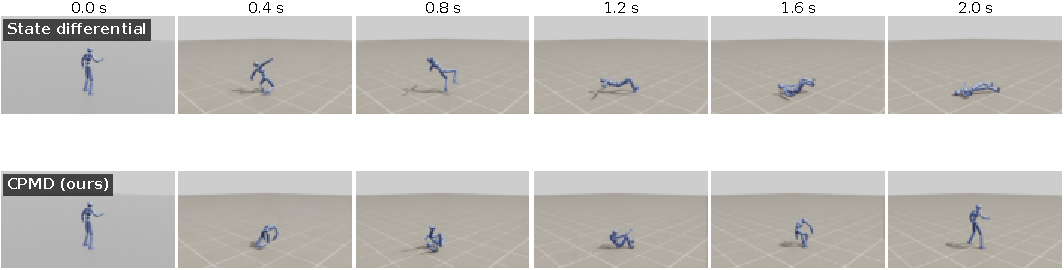
\includegraphics[width=\linewidth]{roll_teaser.pdf}
  \caption{A low-error trajectory need not reproduce the defining behavior.
  The instantaneous differential baseline follows part of the forward motion
  but accumulates almost no directed Roll.  \ours{} exposes error--context
  interactions absent from a difference-first input; this rollout rejects the
  shortcut.  Both sequences use a phase-zero
  reset, deterministic policy, identical camera, and a 2\,s horizon.}
  \label{fig:teaser}
\end{figure*}

\section{Related Work}
\label{sec:related}

\textbf{Reference-conditioned tracking.}
DeepMimic established reinforcement-learning-based tracking with aligned pose,
velocity, end-effector, and center-of-mass objectives
\cite{peng2018deepmimic}.  UniCon and PHC scale such controllers to large motion
collections and improve generalization or failure recovery
\cite{wang2020unicon,luo2023phc}.  KungfuBot/PBHC adapts tracking tolerances
through bilevel optimization \cite{xie2025kungfubot}, while HIL combines
tracking and adversarial imitation for athletic control \cite{wang2025hil}.
SimPoE couples simulated control to video-conditioned pose estimation
\cite{yuan2021simpoe}, and H2O transfers motion imitation to real humanoid
teleoperation \cite{he2024h2o}.  These systems advance controller scale,
robustness, conditioning, or deployment.  Our concern is complementary: the
information retained by a synchronized reference--policy representation before
it is scored.  Learned differential discriminators already replace a manually
aggregated tracking reward with a nonlinear score over a zero-centered paired
error \cite{zhang2025add}.  We retain the adversarial objective and scalar
reward mapping while altering the representation they receive.

\textbf{Motion priors and reusable representations.}
GAIL learns rewards through occupancy matching \cite{ho2016gail}.  MCP composes
learned primitives, and NPMP compresses expert policies into a reusable latent
motor module \cite{peng2019mcp,merel2019npmp}.  AMP learns adversarial style
priors from unstructured clips \cite{peng2021amp}; ASE and CALM extend this
paradigm with reusable or directable embeddings
\cite{peng2022ase,tessler2023calm}.  PULSE distills a large motion imitator into
a universal latent space \cite{luo2024pulse}, MaskedMimic formulates versatile
control as masked motion inpainting \cite{tessler2024maskedmimic}, and ADP uses
temporal dynamics features without explicit phase-aligned pose tracking
\cite{lee2026adp}.  These methods capture broad behavioral context.  We instead
retain synchronized correspondence to one prescribed motion and change only how the
paired histories are differenced.

\textbf{Motion representations.}
Continuous rotation coordinates and exponential maps provide stable local
geometry for articulated motion learning \cite{grassia1998rotations,
zhou2019continuity}.  Bilinear maps expose pairwise feature interactions in a
variety of representation-learning settings \cite{lin2015bilinear}.  We use a
fixed stateless quadratic map for a specific purpose: encode each causal
motion summary before taking the reference--policy difference.

\section{Method}
\label{sec:method}

\subsection{Differential Adversarial Tracking}

Conventional tracking rewards manually aggregate terms such as pose, velocity,
and end-effector error.  Differential adversarial tracking instead places the
complete synchronized tracking differential at the input of a learned
discriminator \cite{zhang2025add}:
\begin{equation}
 \begin{aligned}
 \Delta_t^s&=\phi(\hat s_t)\ominus\phi(s_t),\\
 \mathcal J_D={}&\tfrac12\log D_\theta(0)
 +\tfrac12\mathbb E_{\Delta\sim q_\pi}
   \log\!\left[1-D_\theta(\Delta)\right]
 -\lambda_{\rm GP}\mathcal L_{\rm GP},\\
 r_t={}&-\beta\log\!\left[1-D_\theta(\Delta_t^s)\right].
 \end{aligned}
 \label{eq:objective}
\end{equation}
Here $\phi$ constructs the synchronized state features, $\ominus$ denotes the
appropriate coordinate-wise difference, and the discriminator maximizes
$\mathcal J_D$.  The distribution $q_\pi$ is the empirical mixture of current
and replay policy differentials used by our shared implementation.  The exact
match remains the single positive sample at the origin.
Equation~\eqref{eq:objective} is the learning backbone retained in all of our
comparisons; our method changes only the differential supplied to it.

This elegant zero-centered construction also makes its information boundary
precise.  Let $x^r$ and $x^\pi$ be any additive coordinate block of the aligned
features, with $\Delta_x(x^r,x^\pi)=x^r-x^\pi$.  For every common shift $c$,
\begin{equation}
 \Delta_x(x^r+c,x^\pi+c)
 =x^r-x^\pi
 =\Delta_x(x^r,x^\pi).
 \label{eq:bottleneck}
\end{equation}
Consequently, every scorer $f(\Delta_x)$ is constant over the entire family
$(x^r+c,x^\pi+c)$.  Network depth and width cannot distinguish members of this
family because they are represented by exactly the same input.  In motion
imitation, $c$ corresponds to a common operating regime: the same tracking
error can occur while both trajectories are nearly stationary or while both
carry large coordinated motion.

We therefore alter the representation while retaining the adversarial training
objective and scalar reward mapping: apply the same causal operator to each
side, encode both outputs, and subtract only afterward.  The construction must
remain exactly zero under perfect tracking and use no future states.

\begin{figure*}[!t]
  \centering
  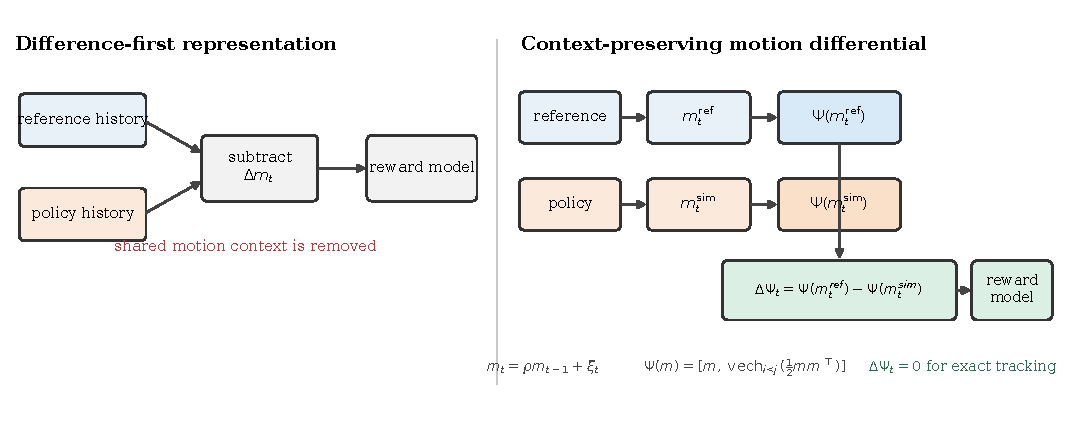
\includegraphics[width=\linewidth]{method_overview.pdf}
  \caption{Difference-first objectives remove common-mode information before
  reward learning.  \method{} summarizes and encodes each history in the same
  fixed frame, then subtracts.  The training objective and scalar reward remain
  unchanged.}
  \label{fig:overview}
\end{figure*}

\subsection{A Causal Motion Summary}

For side $a\in\{r,\pi\}$, let $p_t^a$, $R_t^a$, and $Q_t^a$ denote root
position, root orientation, and articulated joint rotations.  The evaluated
summary uses the same developed increment and discounted accumulator on both
sides:
\begin{equation}
 \begin{aligned}
 \xi_t^a&=
 \begin{bmatrix}
 C_0(p_t^a-p_{t-1}^a)\\
 C_0\Log(R_t^a(R_{t-1}^a)^{-1})\\
 \Log_{\mathcal J}((Q_{t-1}^a)^{-1}Q_t^a)
 \end{bmatrix}\in\R^{d_\xi},\\
 m_t^a&=e^{-\Delta t/\tau}m_{t-1}^a+\xi_t^a,
 \qquad m_0^a=0.
 \end{aligned}
 \label{eq:motion-summary}
\end{equation}
$C_0$ is the inverse heading of the reference at phase zero and remains fixed
for the episode.  Root translation and spatial rotation therefore share one
motion-anchored frame even when the character later becomes horizontal or
inverted.  $\Log_{\mathcal J}$ maps each joint increment to tangent
coordinates, using the joint axis for hinges and exponential coordinates for
spherical joints.  Quaternion representatives are selected on the shortest
branch before taking the logarithm.  These are per-control-step displacements,
not finite differences of an already mixed observation vector.

Using one fixed anchor is important for Roll.  Recomputing heading from the
current root orientation becomes ill-conditioned near inversion and can
inject artificial sign changes.  The fixed anchor is also equivariant to a
common world translation and heading rotation: recomputing it from the
transformed reference gives identical developed increments.

Here $\tau$ is the sole memory-scale parameter, expressed in seconds.  The
decay assigned to a physical lag $\ell$ is $e^{-\ell/\tau}$ regardless of
control frequency.
The implementation stores only $m_t^r$ and $m_t^\pi$; it does not retain a
sequence buffer or recurrent second-order state.

At reset, both accumulators are zeroed and both previous poses are initialized
from the same aligned reference state.  The first nonzero increment is
therefore the first genuine post-reset transition, and partial resets modify
only the corresponding parallel environments.  For cyclic motion, unwrapped
root displacement is used across the reference boundary so that wrapping does
not create a false teleport.

\subsection{Context-Preserving Differential}

We encode each summary with its linear coordinates and one copy of every
cross-coordinate quadratic interaction, then append the history differential
to the instantaneous differential in Eq.~\eqref{eq:objective}:
\begin{equation}
 \begin{aligned}
 \Psi(m)&=\left[m;\triu\!\left(\tfrac12mm^\top\right)\right],\\
 \widetilde\Delta_t&=
 \left[\Delta_t^s;\Psi(m_t^r)-\Psi(m_t^\pi)\right].
 \end{aligned}
 \label{eq:representation}
\end{equation}
Here $\triu(M)=\{M_{ij}\}_{i<j}$ denotes the strict upper triangle.
The linear component ensures that the history block is zero if and only if
$m_t^r=m_t^\pi$.  The quadratic component does not create a competing target;
perfect tracking still produces $\widetilde\Delta_t=0$ exactly.

The extra information is visible in closed form.  Define
$\Delta m=m^r-m^\pi$ and $\Sigma m=m^r+m^\pi$.  The quadratic differential is
\begin{equation}
 \Delta S
 =\tfrac14\triu\!\left(
 \Delta m\,\Sigma m^\top+\Sigma m\,\Delta m^\top\right).
 \label{eq:context}
\end{equation}
Equation~\eqref{eq:context} follows by expanding the two outer products.  It
shows that \method{} exposes pairwise interactions between the tracking
differential and the motion common to reference and policy.  Two pairs may
share the same $\Delta m$ while producing different $\Delta S$ because their
$\Sigma m$ differs.  The scorer can therefore condition an error on the motion
regime in which it occurred.
Here ``context-preserving'' has a specific scope: selected common-mode
interactions survive differencing.  The representation is not a lossless
encoding of either trajectory or of the complete common summary.

\paragraph{A two-dimensional example.}
The information difference does not require a complicated trajectory.  Let a
reference summary be $(1,0)$ and a simulated summary be $(0,0)$.  Their
first-order differential is $(1,0)$, while their only strict-upper quadratic
coordinate has zero differential.  Now add the same context $(0,1)$ to both
summaries.  The new pair is $(1,1)$ and $(0,1)$: its first-order differential
remains exactly $(1,0)$, but its quadratic differential becomes $1/2$.  A
difference-first scorer must assign both pairs the same input.  \method{} can
distinguish them because the same error now co-occurs with motion in the second
channel.  The humanoid construction uses this mechanism across root and joint
increments rather than abstract coordinates.

The evaluated map packs each unordered cross-coordinate product once and
omits self-products.  This indexing is an implementation choice, not a
separate methodological claim; the encode-before-difference principle does
not require dropping the diagonal.  For the humanoid used here,
$d_\xi=3+3+28=34$, giving $d_\xi(d_\xi-1)/2=561$ cross-coordinate terms.
Together with the 172-D instantaneous differential, the discriminator input is
767-D.  The recurrent state remains two 34-D vectors; the quadratic block is
materialized statelessly when the current observation is constructed.

\begin{table}[!t]
\centering
\caption{Information exposed by the evaluated representations.  ``Context''
means selected dependence on the common summary $\Sigma m$, not lossless
recovery of that summary.}
\label{tab:representation}
\begin{tabular}{lcccc}
\toprule
Input & State & History & Context & Dim.\\
\midrule
Instantaneous & \checkmark & -- & -- & 172\\
First-order history & \checkmark & \checkmark & -- & 206\\
\ours{} & \checkmark & \checkmark & \checkmark & 767\\
\bottomrule
\end{tabular}
\end{table}

Table~\ref{tab:representation} separates temporal memory from contextual
encoding.  L1 already uses the same causal accumulator, so the L1--\method{}
comparison does not merely ask whether history helps.  It asks whether
independently encoding the two histories before differencing changes the
learned objective.  The comparison does not hold input width fixed;
Sec.~\ref{sec:cost} states the matched-width control needed for that stronger
conclusion.

\subsection{One Differential, One Reward}

We substitute $\widetilde\Delta_t$ from Eq.~\eqref{eq:representation} for
$\Delta_t^s$ in Eq.~\eqref{eq:objective}; nothing else is added to the policy
objective.  With $D_\theta=\sigma(z_\theta)$, the implemented reward is the
nonnegative capped form
$\beta\min\{\softplus(z_\theta(\mathcal N(\widetilde\Delta_t))),
-\log 10^{-4}\}$.  Away from the numerical cap, this is exactly the reward in
Eq.~\eqref{eq:objective} after the stated replacement and normalization.  Thus
training still has one exact-zero positive, one
negative batch formed from current and replay differentials, one
feed-forward discriminator, and one scalar imitation reward.  There is no
separate trajectory reward, auxiliary branch loss, or modified termination.

The implementation evaluates $D_\theta$ on a scale-normalized differential
$\mathcal N(\widetilde\Delta_t)$, where $\mathcal N(0)=0$ and no running mean is
subtracted.  The original formulation regularizes discriminator gradients at
policy differentials \cite{zhang2025add}; our shared implementation instead
uses a two-endpoint \emph{logit}-gradient penalty at the zero anchor and sampled
policy differentials, plus an $\ell_2$ penalty on the final logit weights.  This
fixed variant is identical in L1 and \method{} and is not part of the proposed
representation.

The classifier objective should not be confused with a behavior metric.
Perfect positive/negative classification only states that zero and the current
policy distribution are separable; it does not show that the reward varies
smoothly over policy-reachable states or that the target motion has been
completed.  We therefore evaluate behavior with winding and inspect policy
reward statistics in addition to discriminator accuracy.

\paragraph{Correctness checks.}
The implementation follows the control-step boundary explicitly.  Immediately
before physics it stores the previous reference and simulated poses.  After
physics, the reference advances to the same new time as the simulator and one
increment is pushed to each accumulator.  The history differential is copied
into the rollout record before reset modifies environment buffers.  This
ordering avoids both a one-step reference offset and a false transition between
episodes.

Correctness tests verify that perfect tracking gives exact zero, the history
encoding is invariant to common world translation and heading, $q$ and $-q$
give identical increments, partial resets do not alter other environments,
and Eq.~\eqref{eq:context} matches the indexed implementation.  These checks
establish formula--code agreement; policy quality is evaluated independently.

\section{Experiments}
\label{sec:experiments}

\subsection{Setup}

\textbf{Simulation and training.}
Experiments use a 15-body humanoid in Isaac Lab \cite{mittal2023orbit} at
30\,Hz control frequency.  The actor and critic are two-layer MLPs with 1024
hidden units; the discriminator is a $1024$--$512$ MLP.  Policies are optimized
with PPO \cite{schulman2017ppo} using 4096 parallel environments, 32-step
rollouts, discount $0.99$, GAE $0.95$, and a 131.072M-sample budget.  The
discriminator uses gradient-penalty weight 2, logit regularization 0.01, and a
replay buffer.  Differential normalization tracks per-coordinate absolute
scale without mean subtraction and freezes after $10^8$ samples.

The reference-conditioned actor sees target frames at the next three control
steps in every compared arm.  Random phase reset is enabled.  All
representation comparisons use the same controller, optimizer, reward
mapping, sample budget, and seed; only the discriminator input differs.

\textbf{Roll task.}
The reference lasts 2.0\,s and contains one full forward Roll with 0.902\,m
root displacement.  Training episodes contain one cycle (60 control steps),
while deterministic evaluation lasts 10\,s (five cycles, 300 steps).  Pose
termination is disabled and all body contacts are allowed.  This is necessary
for the intended ground maneuver, but it also means episode length is always
the configured horizon and cannot serve as success.

\textbf{Compared representations.}
The primary controlled comparison is between: (1) a first-order causal input
$[\Delta_t^s;m_t^r-m_t^\pi]$ (L1), and (2) \ours{} from
Eq.~\eqref{eq:representation}.  Both use $\tau=32/30$\,s and the unchanged
objective in Eq.~\eqref{eq:objective}.  We additionally show an instantaneous
state-differential checkpoint as a qualitative reference.  That checkpoint
was trained with a shorter 65.5M-sample budget, so it is not used for an
equal-budget causal claim.

\textbf{Protocol integrity.}
L1 and \method{} were launched from fresh initialization with the same random
seed, 4096 environments, one-cycle training horizon, engine configuration, and
normalizer schedule.  The policy observation is unchanged, so the new history
is available only to the discriminator and reward.  Both use the nonnegative
reward in Eq.~\eqref{eq:objective}; neither receives a handcrafted
winding term, absolute tracking penalty, or failure bonus.  With contact and
pose termination disabled, the policy cannot improve return merely by ending a
bad Roll early.  These controls make L1 versus \method{} a clean test of the
history representation, subject to the input-width limitation discussed
below.

\subsection{Behavior-Level Evaluation}

Framewise pose error cannot determine whether a periodic path was traversed.
We therefore integrate shortest-branch root-rotation increments about a fixed
Roll axis.  If $\delta\theta_k^a$ is the projected increment for reference or
policy side $a$, directed winding is
\begin{equation}
 w=\frac{\sum_{k=1}^{T}\delta\theta_k^\pi}
 {\sum_{k=1}^{T}\delta\theta_k^r}.
 \label{eq:winding}
\end{equation}
Incremental integration is essential because the orientations before and
after a full $2\pi$ rotation are nearly identical.  We classify an evaluation
as a shortcut when $w<0.5$ and retain the continuous winding value.  We also
report forward-displacement ratio, root-height RMSE, and landing-window upright
alignment.  Each history checkpoint is evaluated for 256 deterministic
10\,s episodes; the qualitative instantaneous checkpoint has 128 evaluations.

The evaluation axes are fixed from the reference rather than inferred from the
policy.  The forward axis is the normalized reference root displacement over
one 2\,s cycle, and the Roll axis is its horizontal perpendicular.  Every
increment is projected onto that same axis, including when the policy is
inverted.  This prevents the metric from changing its meaning when the
character heading becomes unreliable.  Root-height RMSE is measured at every
post-step sample.  Upright alignment is evaluated only in the final 0.2\,s
landing window, because averaging uprightness over a correct Roll would
incorrectly penalize its inverted middle phase.

The threshold $w<0.5$ is used as a transparent diagnostic division between the
near-zero and near-reference modes visible in Fig.~\ref{fig:winding-distribution};
it is not used by the policy.  A final multi-seed study should freeze the
threshold before training and report a threshold-sensitivity curve.  Our main
evidence therefore remains the continuous winding distribution, with shortcut
rate serving as an interpretable count of its low-winding mode.

\begin{table*}[!t]
\centering
\caption{Roll evaluation and final training diagnostics.  L1 and \ours{} use
the same seed, 131.072M samples, and 256 ten-second evaluations.  The
instantaneous checkpoint is a shorter-budget qualitative reference.  Lower is
better for errors and shortcut rate; higher is better otherwise.}
\label{tab:roll-results}
\resizebox{0.98\textwidth}{!}{%
\begin{tabular}{lrrrrrrrrrrr}
\toprule
Method & Train samples & Eval. & Wind. mean & Wind. med. & Shortcut & Disp. ratio & Height RMSE & Upright & Root rot. & Root ang. vel. & Samples/s\\
\midrule
Instantaneous differential & 65.5M & 128 & $-0.007$ & $-0.006$ & 100.0\% & 0.221 & 0.343 & 0.0\% & 1.442 & 1.765 & 57,657\\
First-order history (L1) & 131.1M & 256 & 0.035 & $-0.005$ & 100.0\% & 1.085 & \textbf{0.061} & 30.5\% & 0.475 & 1.522 & \textbf{55,159}\\
\ours{} & 131.1M & 256 & \textbf{0.930} & \textbf{0.976} & \textbf{5.9\%} & \textbf{1.143} & 0.082 & 30.5\% & \textbf{0.270} & \textbf{0.951} & 54,165\\
\bottomrule
\end{tabular}}
\end{table*}

\subsection{Does Context Recover the Defining Motion?}

Table~\ref{tab:roll-results} exposes two qualitatively different solutions.
L1 follows forward motion: its displacement ratio is 1.085 and its mean
root-height error is only 6.1\,cm.  Conventional position and height metrics
would therefore make this run look successful.  Yet its mean winding is
0.035, its median is slightly negative, and every evaluation is a shortcut.
The controller has learned to move with the reference without executing the
directed rotation.

Under the same training budget and seed, \ours{} reaches 0.930 mean winding
and a median of 0.976; 241 of 256 evaluations cross the diagnostic winding
threshold.  Root-rotation and root-angular-velocity errors also decrease by
43\% and 38\% relative to L1.  The slightly higher height RMSE is consistent
with actually entering the low and inverted configurations of the reference,
rather than remaining in an easier near-ground shortcut.  Figure~\ref{fig:behavior}
shows that the difference is not an artifact of episode length: all methods
reach the fixed horizon, while their winding distributions occupy distinct
behavior modes.

\begin{figure*}[!t]
  \centering
  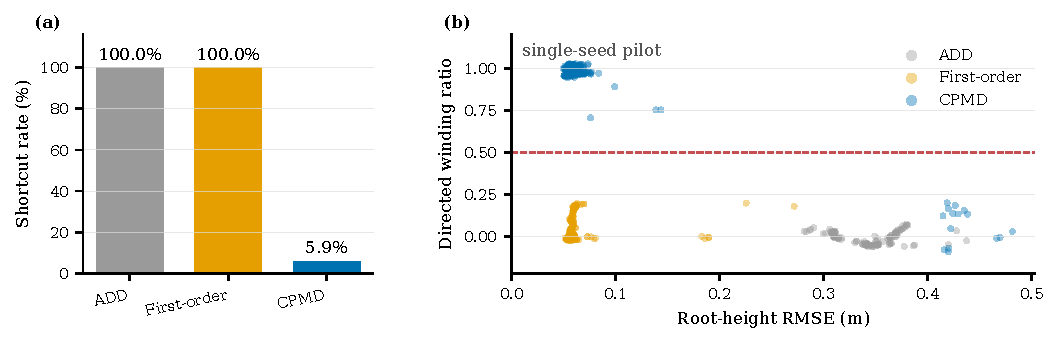
\includegraphics[width=\linewidth]{behavior_summary.pdf}
  \caption{Behavior-level evaluation reveals the non-rolling mode hidden by
  framewise errors.  Bars show shortcut rate; points show directed winding
  against root-height RMSE.  The instantaneous checkpoint is qualitative
  because its training budget differs.  L1 and \ours{} are the controlled,
  equal-budget comparison.}
  \label{fig:behavior}
\end{figure*}

The qualitative rollout in Fig.~\ref{fig:teaser} matches the metrics.  The
instantaneous policy lowers its body and translates but does not complete the
turn.  \method{} enters the contact phase, passes through inversion, and
returns upright.  Since both use identical target observations and legal
contacts, the distinction is attributable to what their reward representation
can expose, not to privileged future input or a hand-coded fall rule.

\begin{figure}[!t]
  \centering
  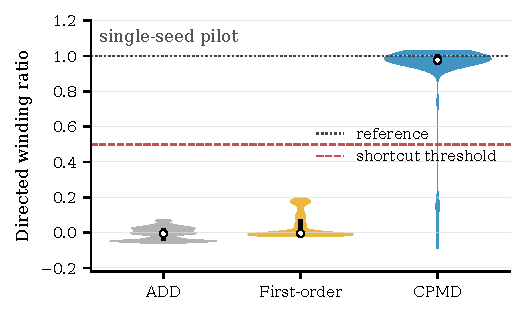
\includegraphics[width=\columnwidth]{winding_distribution.pdf}
  \caption{Distribution of directed winding over the stored deterministic
  evaluations.  L1 concentrates near zero.  \ours{} is concentrated near the
  reference value one, with a small separate failure mode.  The instantaneous
  checkpoint is shown only as a qualitative reference.}
  \label{fig:winding-distribution}
\end{figure}

\subsection{Distribution and Failure Anatomy}

Figure~\ref{fig:winding-distribution} shows why the mean alone is incomplete.
For L1, the 10th, 50th, and 90th winding percentiles are $-0.017$, $-0.005$,
and $0.169$: even its upper tail does not approach one full reference Roll.
For \method{}, the corresponding values are $0.954$, $0.976$, and $1.017$.
The lower mean of 0.930 is caused by a distinct set of 15 low-winding
evaluations rather than a broad tendency to under-rotate.  We therefore report
both continuous winding and the number of low-winding outcomes.

The landing-upright indicator is 30.5\% for both L1 and \method{}.  Thus the
current evidence supports recovery of directed rotation, not a claim that the
controller has solved every landing and stabilization failure.  This
distinction matters: winding tests whether the defining path occurred, while
upright alignment tests a different terminal property.  A controller may pass
one and fail the other.  The final benchmark should report them separately
rather than merging both into one opaque success label.

\subsection{Training Dynamics}

Figure~\ref{fig:training} reports diagnostics at matched environment samples.
Both history methods initially reduce easy translational and posture errors.
L1 continues improving body-position error and eventually reaches a low root
position error, but its root-rotation and angular-velocity curves plateau at a
non-rolling solution.  \method{} undergoes a later transition in the
rotational quantities and finishes with substantially lower errors.  This
behavior explains why a short early-training comparison is misleading: the
defining Roll emerges after the policy has learned enough contact control to
cross the rotational barrier.

\begin{figure*}[!t]
  \centering
  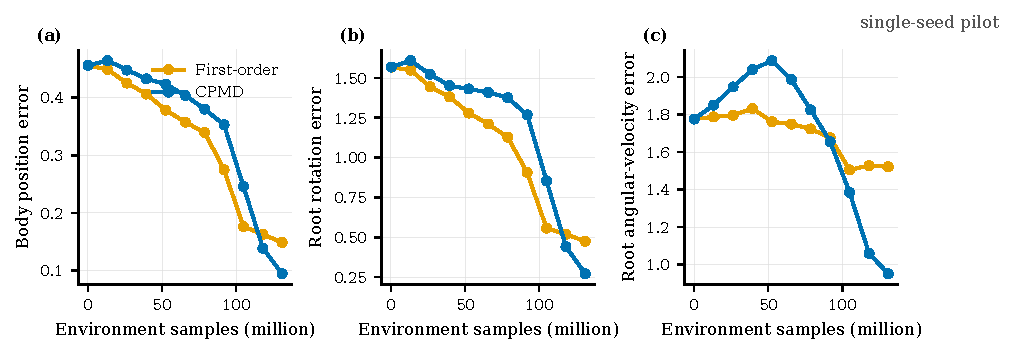
\includegraphics[width=\linewidth]{training_curves.pdf}
  \caption{Training diagnostics versus environment samples.  First-order
  history improves several framewise quantities while remaining in the
  non-rolling mode.  \ours{} exhibits a late improvement in root rotation and
  angular velocity that coincides with the behavioral Roll solution.  Curves
  show one paired training seed and are not confidence intervals.}
  \label{fig:training}
\end{figure*}

The discriminator itself remains a standard zero-versus-policy classifier.
No trajectory-success labels, winding reward, or manually selected Roll axis
enter training; winding is used only for evaluation.  Thus the behavior is not
obtained by directly rewarding the reported metric.  The quadratic block
instead makes motion-regime interactions available to the learned reward.

\subsection{Representation and Computational Cost}
\label{sec:cost}

L1 and \method{} share the same 34-D recurrent state per side.  L1 yields a
206-D discriminator input; \method{} adds 561 stateless cross-channel
coordinates for a 767-D input.  The discriminator grows from 0.737M to 1.312M
trainable parameters, while the actor and critic remain identical.  Measured
throughput changes from 55,159 to 54,165 samples/s, a 1.8\% reduction.  This is
considerably cheaper than maintaining a sequence window or recurrent
second-order state, although rollout and replay storage increase with the
larger discriminator observation.

The current experiment isolates first-order history from the final
context-preserving representation, but it does not by itself separate exposed
common context from every effect of input width and polynomial conditioning.
A decisive final control is a 767-D difference-first input
$[\Delta^s;\Delta m;\triu(\Delta m\Delta m^\top/2)]$.  It has the same width and
quadratic degree but remains a function of $\Delta m$ alone and is therefore
invariant to the common shifts in Eq.~\eqref{eq:bottleneck}.  This control, and
paired training seeds, are required before making a capacity-independent
causal claim.

\subsection{What the Current Evidence Establishes}

Table~\ref{tab:evidence} separates observations from conclusions that require
additional experiments.  This distinction is especially important because
the 256 evaluation episodes share one trained policy.  They measure variation
over evaluation conditions, not the variance of the learning algorithm.

\begin{table}[!t]
\centering
\caption{Evidence boundary of the completed Roll study.}
\label{tab:evidence}
\begin{tabular}{>{\raggedright\arraybackslash}p{0.41\columnwidth}%
                >{\raggedright\arraybackslash}p{0.46\columnwidth}}
\toprule
Question & Current evidence\\
\midrule
Does causal history alone induce Roll? & No in seed 0: L1 has 100\% low-winding outcomes.\\
Does \ours{} avoid that mode? & Yes in seed 0: 241/256 exceed $w=0.5$.\\
Does it solve stable landing? & Not shown: upright rate remains 30.5\%.\\
Is the gain independent of width? & Pending matched-width subtract-first control.\\
Is it robust across training? & Pending paired multi-seed runs.\\
Is it general across motions? & Pending easy and contact-rich tasks.\\
\bottomrule
\end{tabular}
\end{table}

Two completed observations are nevertheless decisive for the stated pilot
question.  First, a low state error and accurate displacement do not imply the
reference Roll occurred: L1 directly demonstrates that combination.  Second,
adding the independently encoded quadratic block changes the learned solution
under one otherwise aligned training run.  Neither observation requires
calling the method state of the art or claiming that input capacity has been
fully controlled.

The mechanism suggested by Eq.~\eqref{eq:context} is also narrower than generic
``long-term reasoning.''  \method{} does not store the full sequence, infer a
symbolic action phase, or supervise path order.  Its accumulator summarizes
recent developed motion, and the quadratic block lets the current mismatch be
evaluated relative to that common summary.  For Roll, this exposes whether
root and joint discrepancies occur while both sides carry the coordinated
motion of the maneuver or while the character follows a low-motion shortcut.
The experiment supports the usefulness of this context; it does not claim a
lossless trajectory representation.

\subsection{Final Statistical Protocol}

The paper-ready comparison will treat the training seed, rather than an
environment or evaluation episode, as the statistical unit.  Each primary arm
will use paired seeds, identical initialization protocol, the same 131.072M
sample budget, and the same checkpoint-selection rule.  We will report
seed-level mean and standard deviation, paired effect sizes, and confidence
intervals for winding, shortcut rate, pose errors, and throughput.  Evaluation
conditions, threshold, phase/reset schedule, and perturbations will be fixed
before launching the final runs.

The minimum primary matrix contains four representations: instantaneous state,
L1, the matched-width subtract-first quadratic control, and \method{}.  A
conventional motion already solved by the instantaneous representation checks
that added context does not degrade easy tracking; a second contact-rich,
path-dependent motion checks whether the Roll result transfers.  These runs
complete the causal and generality claims without changing the method or
introducing another reward component.

\subsection{Scope and Limitations}

The present results establish a large within-seed mechanism result on one
motion, not universal superiority.  Evaluation episodes from one checkpoint
measure conditional behavior variation; they do not replace independent
training seeds.  A final statistical study must repeat the instantaneous,
matched-width, L1, and \method{} arms over paired seeds at the same budget.  It
must also include an action already solved by the simpler representation to
test non-degradation and another contact-rich path-dependent action to test
breadth.

The representation has structural limits.  The discounted accumulator can
alias distinct old histories through cancellation, and the strict-upper map
omits diagonal self-interactions.  The $O(d_\xi^2)$ lifted width may become costly
for much larger motion summaries.  Finally, a better reward representation
does not guarantee that finite-budget PPO will discover every dynamically
difficult maneuver.  These limitations concern the scope of the method, not
the Roll metric: directed winding directly verifies whether the defining
rotation occurred.

\section{Conclusion}

We presented context-preserving motion differentials, an objective-preserving
encode-before-difference representation for adversarial motion imitation.
By encoding reference and simulated histories independently, the method keeps
phase-aligned correspondence while exposing selected interactions between
tracking error and the shared motion regime.  It changes neither the adversarial
objective nor the scalar policy reward.  In a controlled Roll experiment,
first-order history produced accurate displacement but no directed rotation,
whereas \method{} avoided the low-winding shortcut in 94.1\% of evaluations.
More broadly, the result shows why behavior-level path metrics and
representation-level context
are both necessary when low framewise error can hide the wrong motion.

\IEEEtriggeratref{15}
\bibliographystyle{IEEEtran}
\bibliography{references}

\end{document}
